% TODO proof-reading
\subsection{\EN{Second example}\RU{Второй пример}}

\EN{Now another simple crackme example}\RU{Еще один простой пример crackme}:

\begin{lstlisting}
public class password
{
	public static void main(String[] args)
	{
		System.out.println("Please enter the password");
		String input = System.console().readLine();
		if (input.equals("secret"))
			System.out.println("password is correct");
		else
			System.out.println("password is not correct");
	}
}
\end{lstlisting}

\EN{Let's load it to}\RU{Загрузим в} IDA:

\begin{figure}[H]
\centering
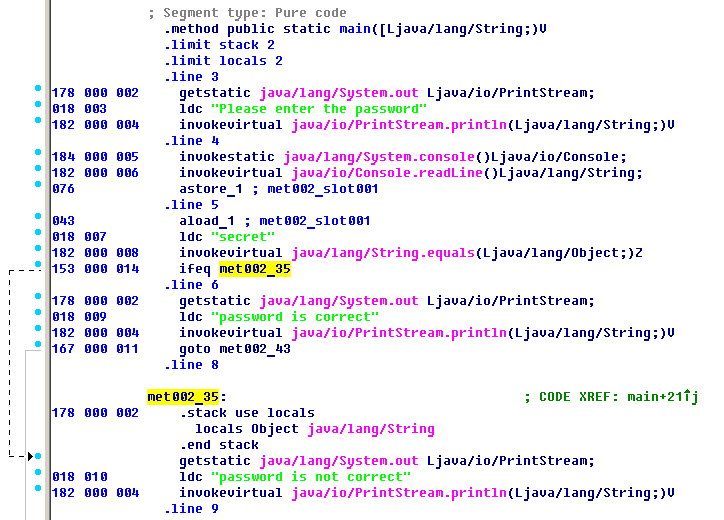
\includegraphics[scale=\FigScale]{Java_and_NET/java/13_patching/2/1.png}
\caption{IDA}
\end{figure}

\EN{We see here \TT{ifeq} instruction which does the job.}
\RU{Видим здесь инструкцию \TT{ifeq}, которая, собственно, всё и делает.}
\EN{Its name stands for \IT{if equal}, and this is misnomer, a better name would be \TT{ifz} (\IT{if zero}), i.e, 
if value at \ac{TOS} is zero, then do the jump.}
\RU{Её имя означает \IT{if equal}, и это не очень удачное название, её следовало бы назвать 
\TT{ifz} (\IT{if zero}), т.е. если значение на \ac{TOS} ноль, тогда совершить переход.}
\EN{In our example, it jumps if password is not correct 
(\TT{equals} method return \TT{False}, which is 0).}
\RU{В нашем случае, переход происходит если пароль не верный 
(метод \TT{equals} возвращает \TT{False}, а это 0).}
\EN{The very first idea is to patch this instruction.}
\RU{Первое что приходит в голову это пропатчить эту инструкцию.}
\EN{There are two bytes in \TT{ifeq} opcode, which encodes jump offset.}
\RU{В опкоде \TT{ifeq} два байта, в которых закодировано смещение для перехода.}
\EN{To make this instruction idle, we must set byte 3 at 3rd byte
(because 3 is to be added to the current address resulting always jump to the next instruction,
since \TT{ifeq} instruction length is 3 bytes):}
\RU{Чтобы инструкция не работала, мы должны установить байт 3 на третьем байте
(потому что 3 будет прибавляться к текущему смещению, и в итоге переход будет на следующую инструкцию,
ведь длина инструкции \TT{ifeq} это 3 байта):}

\begin{figure}[H]
\centering
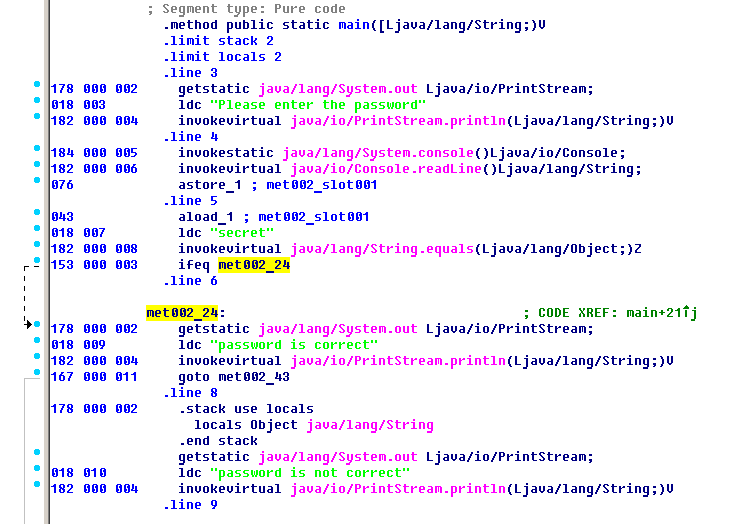
\includegraphics[scale=\FigScale]{Java_and_NET/java/13_patching/2/2.png}
\caption{IDA}
\end{figure}

\EN{That doesn't work}\RU{Это не работает} (JRE 1.7):

\begin{lstlisting}
Exception in thread "main" java.lang.VerifyError: Expecting a stackmap frame at branch target 24
Exception Details:
  Location:
    password.main([Ljava/lang/String;)V @21: ifeq
  Reason:
    Expected stackmap frame at this location.
  Bytecode:
    0000000: b200 0212 03b6 0004 b800 05b6 0006 4c2b
    0000010: 1207 b600 0899 0003 b200 0212 09b6 0004
    0000020: a700 0bb2 0002 120a b600 04b1
  Stackmap Table:
    append_frame(@35,Object[#20])
    same_frame(@43)

        at java.lang.Class.getDeclaredMethods0(Native Method)
        at java.lang.Class.privateGetDeclaredMethods(Class.java:2615)
        at java.lang.Class.getMethod0(Class.java:2856)
        at java.lang.Class.getMethod(Class.java:1668)
        at sun.launcher.LauncherHelper.getMainMethod(LauncherHelper.java:494)
        at sun.launcher.LauncherHelper.checkAndLoadMain(LauncherHelper.java:486)
\end{lstlisting}

\EN{But needless to say, it was worked in}\RU{Хотя, надо сказать, работает в} JRE 1.6.

\EN{We can also try to replace all 3 \TT{ifeq} opcode bytes by zero bytes (\ac{NOP}), 
and it's still doesn't work.}
\RU{Мы также можем попробовать заменить все три байта опкода \TT{ifeq} на нулевые байты (\ac{NOP}), 
но это тоже не работает.}
\EN{Well, probably there are more stack map checks appeared in JRE 1.7.}
\RU{Видимо, начиная с JRE 1.7, там появилось больше проверок карт стека.}

\EN{OK, we'll replace the whole call to \TT{equals} method by \TT{iconst\_1} instruction 
plus pack of \ac{NOP}s:}
\RU{ОК, заменим весь вызов метода \TT{equals} на инструкцию \TT{iconst\_1} плюс набор 
\ac{NOP}-ов:}

\begin{figure}[H]
\centering
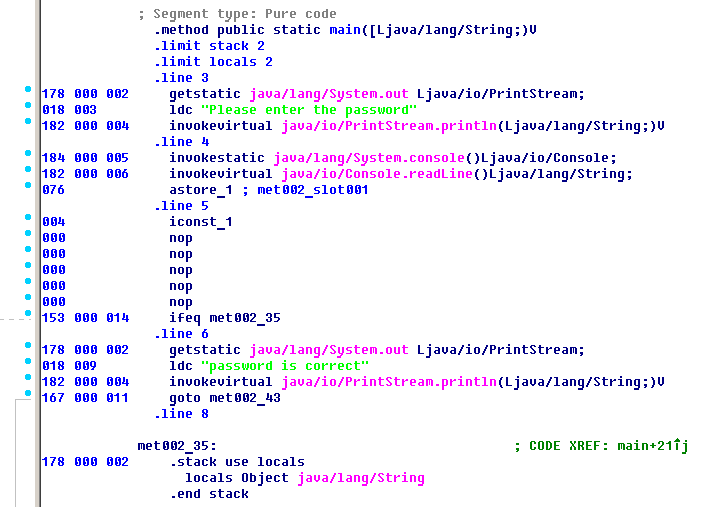
\includegraphics[scale=\FigScale]{Java_and_NET/java/13_patching/2/3.png}
\caption{IDA}
\end{figure}

\EN{1 is always to be at the \ac{TOS} when \TT{ifeq} instruction is executed, 
so \TT{ifeq} will never jump.}
\RU{1 будет всегда на \ac{TOS} во время исполнения инструкции \TT{ifeq}, 
так что \TT{ifeq} никогда не совершит переход.}

\EN{This works}\RU{Это работает}.
